% Metódy inžinierskej práce

\documentclass[10pt,slovak,a4paper]{article}

\usepackage[slovak]{babel}
%\usepackage[T1]{fontenc}
\usepackage[IL2]{fontenc} % lepšia sadzba písmena Ľ než v T1
\usepackage[utf8]{inputenc}
\usepackage{graphicx}
\usepackage{float}
\usepackage{caption}
\usepackage{subcaption}
\usepackage[utf8]{inputenc}
\usepackage{url} % príkaz \url na formátovanie URL
\usepackage{hyperref} % odkazy v texte budú aktívne (pri niektorých triedach dokumentov spôsobuje posun textu)

\usepackage{cite}
%\usepackage{times}

\pagestyle{headings}

\title{Softvér pre DIAbetikov\thanks{Semestrálny projekt v predmete Metódy inžinierskej práce, ak. rok 2021/22, vedenie: Vladimír Mlynarovič}} 

\author{Daniel Brilla\\[2pt]
	{\small Slovenská technická univerzita v Bratislave}\\
	{\small Fakulta informatiky a informačných technológií}\\
	{\small \texttt{xbrillad@stuba.sk}}
	}

\date{\small 12. december 2021}



\begin{document}

\maketitle

\begin{abstract}
Diabetes je v dnešnnom svete už bežnou chorobou, ktorou trpí čím ďalej, tým viac ľudí. Väčšina diabetikov používa bežne dostupné softvéry, ktoré avšak, podľa mojich názorov nedržia krok s dobou. Ponúkajú len dlhodobé sledovanie si hladiny cukru. V digitálnej dobe, plnej umelej inteligencie vieme, opäť podľa mojích názorov, sa dá posunúť vpred a zjednoduchšiť každodenný život. 

\paragraph{Kľúčové slová:} Diabetes, Fuzzy logika, Inteligentný softvér, GIM, Modifikované upozorňovacie skóre 
\end{abstract}



\section{Úvod}

V tejto semestralnej práci sa budem venovať problematike v softvérovom inžinierstve a ako zlepšiť život diabetikom po celom svete. S narastajúcim počtom diabetikov po celom svete prevencia už nepostačuje.
Ja potrebné spraviť krok vpred a tím je zaoberanie sa otázkou, ako v dnešnom modernom svete zlepšiť každodenný život diabetikov? 
Táto problematika nemá také ľahké riešenia ako sa zdá. Teória je mätúca a riešenia sú v aktuálnom stave málo použiteľné.

Na začiatok si povieme čo je diabetes a aké su jeho typy. Následne sa pozrieme na niektoré softvérové riešenia ako GIM a iné.
Nakoniec si všetko zhrnieme a aké sú vízie, poprípade čo sa plánuje do budúcnosti a čo by chceli v budúcich sofvéroch diabetici vidieť. 






\section{Čo je diabetes} \label{diabetes}

Diabetes mellitus je metabolická disfunkcia charakterizovaná hyperglykémiou, ktorá je dôsledkom porúch sekrécie inzulínu z pankreasu, účinku inzulínu alebo spojením oboch porúch.\cite{2004}
Chronická hyperglykémia diabetu je spojená s dlhodobým poškodením, dysfunkciou a zlyhaním rôznych orgánov, najmä očí, obličiek, nervov, srdca a ciev.

Na vzniku cukrovky sa podieľa niekoľko faktorov. Tieto sa pohybujú od autoimunitnej deštrukcie beta buniek pankreasu s následným nedostatkom inzulínu po abnormality, ktoré vedú k rezistenci bunieki na pôsobenie inzulínu.
Porušenie sekrécie inzulínu a defekty v pôsobení inzulínu často koexistujú u rovnakého pacienta a často nie je jasné, ktorá abnormalita, či už samotná, je primárnou príčinou hyperglykémie, prípadnej hypoglykémie.\cite{2004}

Medzi príznaky diabetesu patrí strata hmotnosti, alebo obezita, nadmerné močenie, smäd, hlad. Vážnejšími príznakmi sú napríklad zhoršenie zraku, problémy pri močené a iné.
K dlhodobým komplikáciám diabetu patrí retinopatia s potenciálnou stratou zraku, nefropatia vedúca k zlyhaniu obličiek, periférna neuropatia s rizikom vredov na nohách. U pacientov s diabetom je zvýšený výskyt aterosklerotických kardiovaskulárnych, periférnych arteriálnych a cerebrovaskulárnych chorôb.\cite{2004}

Prevažná väčšina prípadov cukrovky spadá do dvoch širokých etiopatogenetických kategórií. Pri cukrovke 1. typu, je príčinou absolútny nedostatok sekrécie inzulínu. Pri druhej, oveľa rozšírenejšej kategórii, cukrovke typu 2, je príčinou kombinácia odolnosti voči účinku inzulínu a neadekvátnej kompenzačnej sekrečnej reakcie na inzulín.\cite{2004}




\section{Aktuálny softvér pre diabetikov}

Keď si človek otvorí na svojom mobilnom zariadení, notebooku alebo počítači prehľad aplikácii pre diabetokv, všetko čo nájde sú promárne aplikácie určené pre sledovanie a analyzovanie už daných hladín cukru v krvy (glykémie).
Veľká pomoc pre diabetikov, ktorý si so sebou nie vždy berú svoj diabetický denník. Množstvo týchto aplikácii pracuje a komunikuje aj s RFID senzormi, ktoré, môže mať človek na sebe ak ná inzulínovú pumpu alebo senzor na kontinuálne meranie krvy. 
Pomocou týchto softvérov si môže diabetik s pumpou, bez toho, aby robil nejaký zásah, alebo vyberal veci naviac, zmerať glykémiu a v prípade vysokej glykémie aj pripichnúť si inzulín.

Avšak, pri dnešnom modernom svete, ako si povieme neskôr\ref{int-sof}, umelá inteligencia (AI) v kombinácii s doterajšími poznatkami, by sa falo predísť katastrofálnehším stavom a zmierniť vedľajšie komplikácie, ktoré s týmto ochorením idú ruka v ruke.
Nehovorím týmto, že tieto riešenia sú zlé. Podľa mňa sme za 100 rokov liečby diabetesu pokročili o míľové kroky vpred, avšak netreba sa zastaviť. Musíme napredovať a využívať vedomosti nie na zabíjanie ľudí a dokazovanie si moci, ale na pomoc druhým. 
Lebo pravá sila je ukrytá nie v tom, čo človek vie zobrať, ale čo vie druhému dať. A toto platí nielen pri diabetese ale aj pri ostatných, rovnako vážnych ochoreniach. 


\section{GIM} \label{GIM}


GIM alebo Glucose-Insulin Model softvér nám dáva schopnosť simulovať chovanie sa jedinca a jeho sekréciu inzulínu.

V poslednej dobe bol navrhnutý nový model simulácie jedla, ktorý umožnil meranie rôznych tokov, glukózy a inzulínu, vyskitujúcich sa počas jedla. V skutočnosti je systém, veľmi zložitý a iba dostupnosť tokov glukózy a inzulínu, ich plazmatických koncentrácií, nám umožní minimalizovať štruktúrne neistoty pri modelovaní rôznych procesov. Model pozostáva z 12 nelineárnych diferenciálnych rovníc, 18 algebraitických rovníc a 35 parametrov.

 Užívateľsky príjemný simulačný softvér tohto modelu by bol veľkou pomocou, najmä pre vyšetrovateľov bez konkrétnych odborných znalostí v oblasti modelovania.Softvér GIM, implementovaný v MATLAB verzii 7.0.1, ktorý umožňuje simulovať normálne aj patologické stavy, napr. Diabetes typu 2 a inzulín s otvorenou a uzavretou slučkou infúzie pri cukrovke 1. typu. Softvér sa nepokúša riešiť patofyziologické otázky.

\subsection{MATLAB Version}

Keď je GIM spustený, otvorí sa dialógové okno, ktoré čaká od užifvateľa, aby zvolil typ subjektu pre modelovanie. Na výber sú tri možnosti, a to Normálny, typ 2 Diabetik aleb o typ 1 Diabetik.

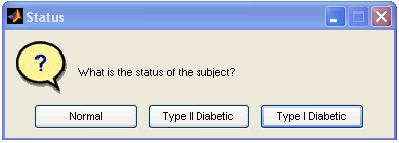
\includegraphics[scale=0.5]{ob-1.PNG}

Keď používateľ klikne na subjekt Normálny alebo Diabetik 2. typu, zobrazí sa interaktívne okno, ktoré je rozdelené na tri časti. 

1. Bazálne, kde sú stanovené základné hodnoty koncentrácie glukózy, koncentrácie inzulínu a produkcie glukózy. Kliknutím na tlačidlo VÝPOČET sa vypočíta bazálna hodnota glukózy a zobrazí sa na príslušnom štvorci 

2. Subjekt, kde sú hodnoty telesnej hmotnosti a hlavné metabolické indexy, ako sú periférna a hepatálna citlivosť na inzulín (Vmax a kp3, v tomto poradí), dynamická a statická odozva beta-buniek na glukózu (K a beta, v tomto poradí ), sa zadávajú ako percento bežných hodnôt12; pre diabetické subjekty typu 2 sa spočiatku zobrazia typické odchýlky. 

3. Protokol, kde je nastavený čas troch jedál a množstvo prijatej glukózy. 

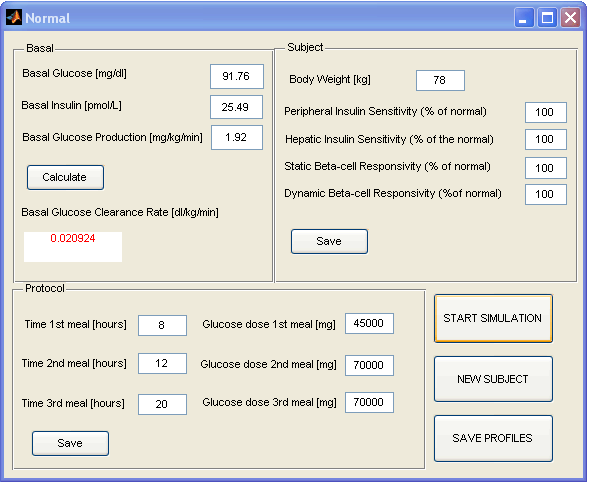
\includegraphics[scale=0.5]{ob-2.PNG}

Akonáhle sú všetky polia nastavené a nové hodnoty sú uložené, simulácia sa spustí kliknutím na START SIMULATION. Výsledky simulácie sú prezentované v grafickom formáte, tj. Je zobrazený obrázok, ktorý ukazuje koncentrácie glukózy a inzulínu, produkciu glukózy, využitie glukózy, vzhľad jedla a sekréciu inzulínu.

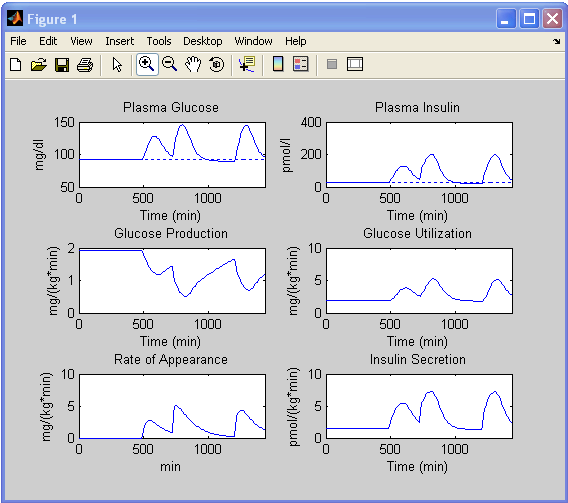
\includegraphics[scale=0.5]{ob-3.PNG}

Keď požívateľ zvolí  Diabtik 1. typu, okno je o trochu inšie, pridá sa tam jedna sekcia.

4. Kontrola, ktorá umožňuje užívateľovi vybrať, či je subjekt kontrolovaný v otvorenej slučke alebo v uzavretej slučke s regulátorom PID. Ak je zvolená otvorená slučka, je možné zadať rýchlosť infúzie bazálneho inzulínu. Ak je zvolená uzavretá slučka, užívateľ môže zvoliť bazálnu koncentráciu inzulínu, ktorý musí tiež definovať cieľovú hodnotu glukózy. 

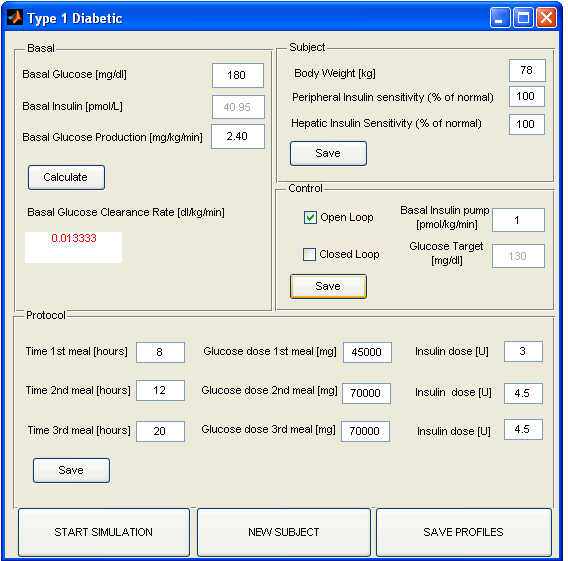
\includegraphics[scale=0.5]{ob-4.PNG}

Program taktiež umožňuje ukladať si profily a výsledky v .mat typoch súborov, stalčením SAVE PROFILES.

Softvír GIM umožňuje taktiež porovnávanie výsledkov medzi normálnym, zdravím jedincom a Diabetikom 1. typu, poprípade rôznej kombinácii 2 subjektov.

\section{Inteligentný softvér} \label{int-soft}

V tejto kapitola sa budeme venovať kapitole z knihy Diabetes Technology and Therapeutics\cite{2000}, ktorá ma zaujala kapitolou o inteligentnom diabetickom softvéry.

Pre diabetikov prvého typu je ťažké udržať si stálu alebo optimálnu hladinu cukru \ref{diabetes}. Riešením by bol systém umelej inteligencie pozostávajúci z liečebných algoritmov kalibrovaných prostredníctvom veľkých súborov údajov špecifických pre pacienta.\cite{2000} Znie to zaujímavo, ale chybičku vidím v tom, ako sa ďalej píše v knihe, že je to potrebné spraviť po každej zmene, či už denného režimu, inzulínu alebo športových aktivít. Samotné nastavenie systému nie je v prototype jednoduché a pre množstvo užívateľov neprípustné. 

Softvérový prototyp založený na neurónovej sieti, fuzzy logike a konceptoch expertného systému bol vyvinutý a hodnotený na určenie uskutočniteľnosti a účinnosti predikčného modelu špecifického pre pacienta. Priemerná absolútna percentuálne chyba medzi skutočnými a predpokladanými hodnotami glykémie (hladiny cukru v krvi) zo vstupov denného inzulínu, jedla a informácií o cvičení u testovacích subjektov s Diabetes Melitus 1 bola 10.5 percenta.\cite{2000}
Zdá sa to ako celkom veľká odchýlka, čo aj je, avšak je to stále dosť presné nato, aby to dokázalo zabrániť životu nebezpečným situáciám. 

\subsection{Fuzzy Logika v zdravotníctve}

Typickému zhoršeniu stavu u chorých ľudí predchádzajú rôzne fyziologické zmeny ako pulz alebo krvný tlak. Modifikované upozorňovacie skóre je systém, ktorý bol vyvinutý na assistenciu nemocničnému personálu pri meraní týchto zmien a pri identifikácii pacientov, ktorý potrebujú naliehavú lekársku pomoc aby sa predišlo katastrofálnym stavom. \cite{2019} Systém je aktuálne implementovaný a testovaný v Rashid Center for Diabaetes and Research v UAE.

Primárne požiadavky systému je diaľkový zber vitálnych funkcií pacienta, ktoré sa merajú pomocou snímačov na báze RFID a hodnotenie zdravotného stavu pacienta pomocou algoritmov založených na fuzzy logike.  Tieto dáta sú následne uchované v elektronických lekárskych záznamoch (EMR) a upozorniť zdravotnícky personál o pacientovom statuse a či potrebuje urgentnú starostlivosť alebo nie. \cite{2019} Následný diagram\ref{schema} nám ukazuje schému navrhovaného systému.

\begin{figure}[H]
\centering
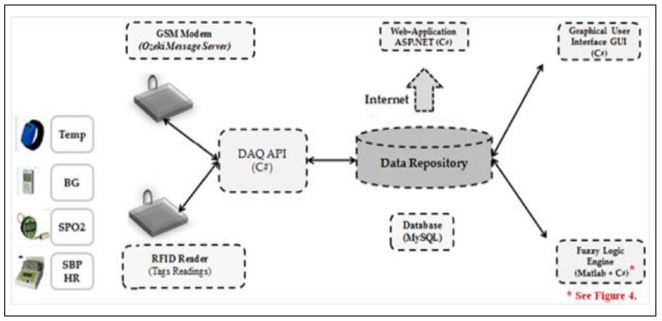
\includegraphics[scale=0.75]{scheme-fuzzy.png}
\caption{Schéma navrhovaného systému \cite{2019}}
\label{schema}
\end{figure}

RFID senzory môžu komunikovať bezdrôtovo s mobilným zariadením a následne pomocou mobilnej siete prenášať informácie do centrálneho monitorovacieho systému - počítača. Tento systém umožňuje implementáciu viacerých užívateľov ako aj počet oblastí monitorovania. \cite{2019} 

Systém pozostáva z rôznych softvérových modulov. Ide o tieto moduly: programovateľné rozhranie pre jednotku zberu dát – aplikácia (DAQ-API), fuzzy logic engine (FLE), databázový manažér (DM), grafické používateľské rozhranie (GUI) a webová aplikácia (Web- Aplikácia).\cite{2019} Podrobnosti a funkcie každého softvérového modulu nájdete v tomto článku \cite{2019}. 

\begin{figure}[H]
\centering
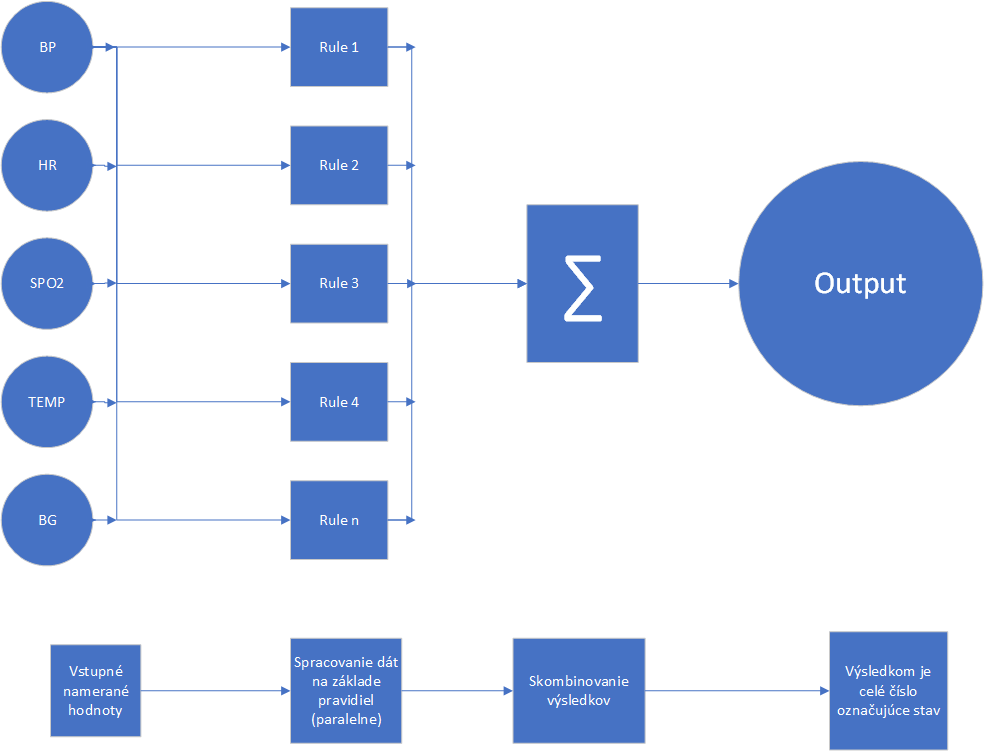
\includegraphics[scale=0.5]{rule-based-engine.png}
\caption{Prekreslená schéma fuzzy procesu podľa článku\cite{2019}}
\label{fuzzy}
\end{figure}

V schéme \ref{fuzzy} vstupujú dáta z RFID senzorov a výsledkom je jedno číslo (status) stavu pacienta. Paralelný charakter pravidiel je jedným z dôležitejších aspektov systémov fuzzy logiky. Namiesto ostrého prepínania medzi režimami na základe bodov prerušenia, logika plynulo prúdi z oblastí, v ktorých správaniu systému dominuje jedno alebo druhé pravidlo. Systém je implementovaný pomocou MATLAB Fuzzy Logic Toolbox. \cite{2019}

\subsection{zhrnutie}
Inteligntné systémy sú riešením avšak s technológiou prichádza aj daň. Systém sa zdá byť na povrchu jednoduchý avšak pre čo najrýchlejšie spracovanie údajov je potreba celkom veľké množstvo výpočtovej techniky a to nerozprávam len o počítačoch na výpočet. Senzory nevydržia dlho. Abbott FreeStyle Libre, čipy, senzory pre kontinuálne sledovanie hladiny cukru, tiež nevydržia večne. A ďalšou požiadavkou bolo pripojenie na mobilnú sieť aby sa dáta dali nahrať na webstránku. Toto je síce menší problém, keďže dáta sa dajú ukladať lokálne a následne naraz odoslať do systému pre spracovanie. Je tam pár háčikov ale blížime sa.


\section{Záver} \label{zaver}
Na koniec si zhrňme, čo sme si v tejto práci opísali. Diabetes je choroba, ktorá v dnešnej dobe nemá riešenia a jedine ako ju zvládnuť je jednoducho prijať to. Avšak riešením by mohli byť moderné technológie a umelá inteligencia.
Vďaka výdobitkom modernej doby môžeme zlepšiť životný štýl tisícom a možno i miliónom ľudí, ktorý toutu zákernou chorobou trpia.

Nakoniec len toľko, že ako jeden diabetikov, si uvedomujem vážnosť situácie a je to neustáli, každodenný boj.
Preto môžem povedať, využime výdobitky našej doby na pomoc druhým a nie na to, aby sme sa ich zbavovali. % prípadne iný variant názvu



%\acknowledgement{Ak niekomu chcete poďakovať\ldots}


% týmto sa generuje zoznam literatúry z obsahu súboru literatura.bib podľa toho, na čo sa v článku odkazujete
\newpage
	\bibliography{literatura1.bib}
	\bibliographystyle{ieeetr} % prípadne alpha, abbrv alebo hociktorý iný
\end{document}
